\chapter{Design and Fabrication} 
\label{3}
The idea of this microfluidic platform is to design a housing package with flexible built in microchannels. As illustrated in \autoref{1_2_1} and as is shown in \autoref{figure3_1}, the suspension is supposed to flow in a microchannel with well-defined variable depth so that the hydrodynamic environment is controllable and quantifiable. In this thesis work the microfluidic platform design, fabrication and integration are the main task and initial pressure and leakage tests are also conducted. However, the study of adhesion features of the bacteria is not included due to time limit.

\begin{figure}[ht]%
\centering
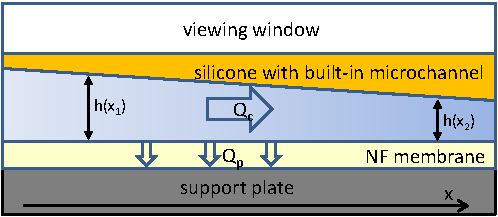
\includegraphics[width=0.6\textwidth]{figures/designandfabrication/figure3_1}%
\caption{Schematic design of the integrated structures in the microfluidic platform}%
\label{figure3_1}%
\end{figure}

To observe the filtration features during separation, the channels in which the suspension flows should be visible. Therefore the housing for the silicone channels and the nanofiltration membrane should be totally optically transparent. Moreover, because this microfluidic platform is designed also for high pressure applications, a stable sealing of the whole housing under high pressure is needed for the leakproofness. Apart from that, the sealing and packaging procedure must be reusable and resealable in order to provide the possibility of assembling and disassembling of the housing many times to replace the nanofiltration membranes. \\

In this chapter, the basic information of nanofiltration membranes and the advantages of using silicone membranes as a basis for sealing gaskets are explained and discussed. Also, the fabrication steps of the silicone membranes are introduced. To machine microchannels in these silicone membranes a novel laser processing technology is explained and analyzed, including machining through-cut microchannels and microchannels with variable depth. The flip-chip transferring steps of the silicone microchannel followed to attach the soft silicone membrane with built in microchannels to a glass slide as a carrier are introduced. All the fabrication steps above have been considered to be reproducible and flexible for further developments. At last, several housing designs are performed to assemble the microchannels with nanofiltration membrane to contribute the microfluidic platform and a test setup is designed for pressure and leakage tests of this platform. 

\section{Nanofiltration Membranes}
\label{3_1}
Nanofiltration refers to a special membrane process which rejects particles on the nanometer size scale. The nanofiltration membrane is a type of pressure-driven membrane with properties between those of reverse osmosis (RO) and ultrafiltration (UF) membranes. Nanofiltration membranes have applications in several areas such as water treatment for drinking water production as well as wastewater treatment. They also offer many advantages such as low operation pressure, high flux, and high retention of multivalent anion salts, relatively low investment and low operation and maintenance costs \cite{hilal2004comprehensive}. \\

In this master thesis, the microfluidic platform is built for testing the adhesion features of bacteria when permeate flow is introduced by the nanofiltration membrane. Suspensions containing colloidal particles like bacteria are supposed to be filtered by such nanofiltration membrane when flowing over and the phenomena such as deposition and adhesion as well as bacteria colony growth is to be investigated during and after the filtration. The type of the nanofiltration membrane selected for this test is NF90.

\section{Silicone Microchannels}
\label{3_2}
The microchannels are built in 200~$\mathrm{\mu m}$ thick silicone membranes with an inlet and an outlet reservoir and a 1mm wide microchannel connecting the inlet and the outlet. Because silicone is soft material, this silicone membrane is then glued to a microscope glass slide which acts as the mechanical microchannel carrier.

\subsection{Advantages of Silicone Material }
\label{3_2_1}
In this master work, the type of silicone selected is WACKER Silicone M 4641 A/B. It is composed of two components: silicone compound and platinum catalyst which are mixed with a mass ratio 10:1. The basic technical data is listed in \autoref{table3_1}.\\

\begin{table}[!h]
    \centering
    \caption{Product data of WACKER silicone M 4641 A/B \cite{wackersilicone}}
    \begin{tabular}{ll}
    \toprule
    Typical general characteristics	& Value \\
    \midrule
    Viscosity at ${23}^{\circ}$C & 30000 mPa s \\
    Color & Translucent \\
    Hardness Shore A & 43 \\
    Elongation at break & > 300\% \\
    \bottomrule
    \end{tabular}
    \label{table3_1}
\end{table}

To obtain direct observation of microscopic processes that occur at the nanofiltration membrane surface the transparency of the microchannel is needed. Therefore the microchannel should be built in a material which has good optical transparency and hence this silicone material is applicable here. Apart from that, silicone is non-toxic and does not release any particles; hence the solutions would not get contaminated. Another reason of choosing silicone is its good sealing performance. Silicone can adhere to glass well without additional adhesive by conformal contact and that is also the reason why glass slide is chosen as the microchannel carrier. Silicone also seals well to other material since it can deform to provide leak-free sealing. Last but not the least, stock silicone membranes of a fixed thickness can be cast in a mold. Sections of this stock membrane can then be cut, adhered to a glass slide and laser patterned for multiple chips. \\

\subsection{Advantages of Laser Rapid Prototyping}
\label{3_2_2}
There are already methods to pattern microchannels in silicone materials. One of them is the soft lithography as illustrated in \autoref{2_2_2}. This method relies on the fabrication of the mold, to which the silicone is casted. The fabrication technology for fabricating the mold is photo lithography, which is cleanroom process and needs multiple complex procedures such as mask deposition and patterning. However, any cleanroom processes in this thesis work are supposed to be avoided since they are complicated and time-consuming. Besides, different casting molds are needed for different microchannel designs, leading to low design flexibility and high cost. Therefore, to save time and cost, laser rapid prototyping (LRP) processes are taken into account.\\

A laser is a device that emits light through a process of optical amplification based on the stimulated emission of electromagnetic radiation \cite{ref_4}. Laser cutting is done by focusing a beam of high intensity energy on the material to be cut, which causes it to either melt or evaporate, depending mostly on the laser intensity and the laser pulse width. Laser cutting machines can be classified into two main categories according to the laser wavelength: deep ultraviolet (DUV) (about 200-300nm) lasers and infrared or visible lasers such as CO$_2$ and Nd:YAG lasers (0.5-10$\mu$m). The ablation mechanism of the former lasers is a photochemical process in which the chemical bonds in the material are broken while that of the latter lasers are to heat and melt the material directly \cite{lasermicromachining}. The laser which is available in our lab is a Nd:YAG laser (DPL Smart Marker II from ACI company) . The wavelength of this laser is 1064nm and the pulse length can be adjusted within the range 15-100ns. The pulse repetition rate can also be user-defined from 1 to 100kHz. The basic mechanism of laser cutting of this laser is shown in \autoref{figure3_2} and can be summarized as follows:

\begin{itemize}
	\item A high intensity beam of infrared light is generated by the laser.
	\item This beam is focused onto the surface of the work piece by means of lens.
	\item The focused beam heats the work piece and establishes a very localized melt.
	\item This localized area of work piece is removed thus generating a cut.
\end{itemize}

\begin{figure}[ht]%
\centering
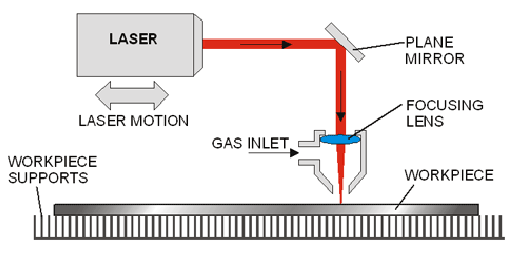
\includegraphics[width=0.6\textwidth]{figures/designandfabrication/figure3_2}%
\caption{Schematic of laser cutting \cite{lasercut}.}%
\label{figure3_2}%
\end{figure}

The machining accuracy of the laser is enough for the work in this thesis. One prominent advantage of LRP is the flexibility. The microchannel models are firstly constructed by computer-aided design and they could be directly subjected to the implementation of LRP. This means the geometric design of the microchannel could be quite flexible and fast. To conclude, the main advantages of LRP can be summarized as follows:

\begin{itemize}
	\item Processing procedures are simplified and fast.
	\item Cost of the processing is low.
	\item Machining precision is acceptable.
	\item Microchannel design is fast and flexible.
\end{itemize}

\section{Silicone Casting}
\label{3_3}
The type of silicone used here is WACKER silicone M 4641 A/B. It is a two-component silicone rubber which vulcanizes at room temperature as mentioned in \autoref{3_2_1}. Component A is the platinum catalyst while component B is the silicone and the mix ratio of the two components is 1:10 (mass). \\

First of all, all the tools and the containers which will be used should be cleaned by acetone and isopropanol. Therefore most of the dusts are removed so that the silicone will not be contaminated.
Then the silicone components A and B are measured with 1:10 weight ratio in a container. A weighing scale is used for the weight measurement. The compounds should be stirred for a few minutes with a spatula until it is thoroughly mixed.\\

The mixture is then placed in a vacuum chamber for degassing since a lot of air is introduced during the stirring. The degassing process lasts for 15 minutes so that the most of the air can be removed from the silicone mixture.\\

After the degassing process the silicone mixture is poured to the casting mold uniformly shown in \autoref{figure3_3}. Then a metal lid is compressed against the silicone by screws and the silicone will fill in all the gaps in the mold. The depth of the casting area is 200$\mu$m and that is the thickness of the cured silicone membrane. After 12 hours (cure time) the mold could be opened and the silicone membrane could be peeled off.\\

\begin{figure}[!t]%
\centering
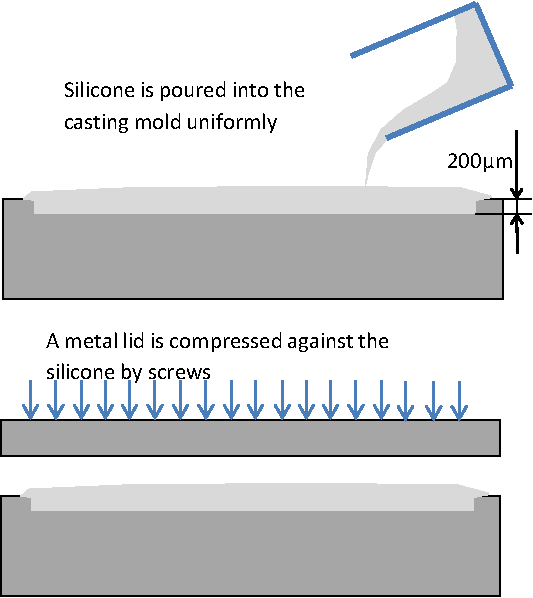
\includegraphics[width=0.6\textwidth]{figures/designandfabrication/figure3_3}%
\caption{Silicone casting steps}%
\label{figure3_3}%
\end{figure}

\section{Design and Fabrication of Silicone Microchannels}
\label{3_4}
The 200$\mu$m thick silicone membranes produced from the former step are at first cut to the size of a glass slide (76 $\times$ 26mm) and attached to the glass slide. The glass slide acts as the mechanical carrier of the membrane because the silicone is too soft. This silicone membrane with glass slide is to be patterned by the laser. \\

The silicone membrane is transparent to the laser so that it does not absorb any laser beam. Therefore it cannot be cut directly. To solve this problem the other side of the silicone is attached to a steel sheet (from H+S Pr\"azisions Folien, CrNi-Stahl, hardness: 1.4310, thickness: 110$\mu$m) which will be ablated first. In this thesis work, this steel sheet is applied to all laser patterning of silicone membrane. Due to the material properties, changing this metal material may result in a change of the laser parameters. \\

When ablated, the metal melts or even evaporates and will release high temperature ablated particles. These particles with certain kinetic energy will diffuse and some of them move towards the silicone membrane and burn the silicone membrane at the same time and thus the silicone membrane is patterned by this indirect laser ablation. The heat energy and the kinetic energy both play a role in the ablation of silicone membrane and define the depth and the quality of the ablation. The main advantage of this indirect ablation is minimized thermal damage to the silicone membrane. Because the laser under use generates long-pulse laser waves, it will heat the adjacent work piece as well rather than just ablate the area where the laser spot focalizes as illustrated in \autoref{2_2_1}. Since steel is a far better thermal conductor than the silicone, the heat in the locally generated hot spot during ablation is quickly transported away, thus the thermal damage to the silicone membrane is reduced. The laser processing flow is shown as \autoref{figure3_4}:\\

\begin{figure}[ht]%
\centering
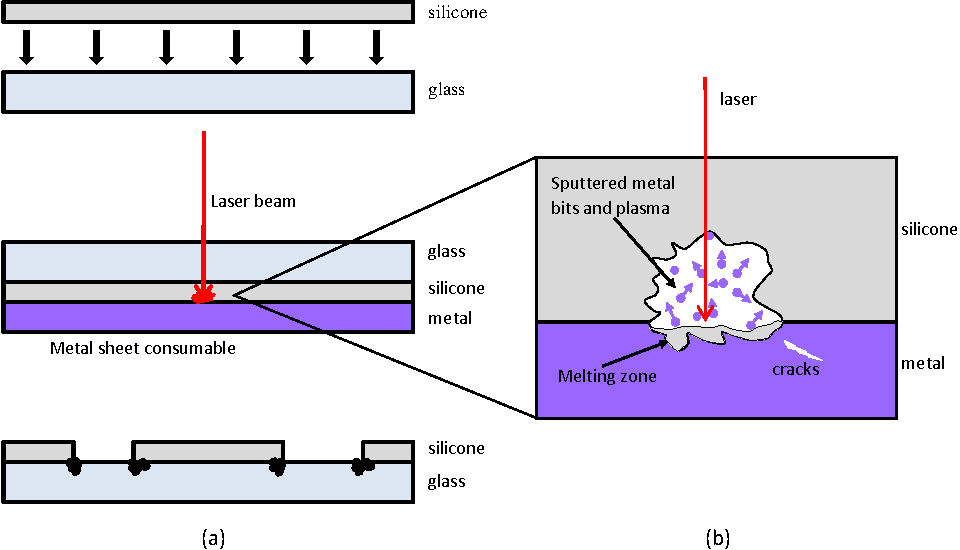
\includegraphics[width=0.8\textwidth]{figures/designandfabrication/figure3_4}%
\caption{(a) Process flow of the silicone machining process, (b) Detail view of the laser working.}%
\label{figure3_4}%
\end{figure}

A jig is designed for the silicone laser processing to hold the glass, silicone and metal layers. The glass with the silicone membrane is compressed to the metal sheet to ensure full contact. This compression is realized by uniformly distributed screws. \autoref{figure3_5} shows the geometry design of the jig.\\

\begin{figure}[t]%
\centering
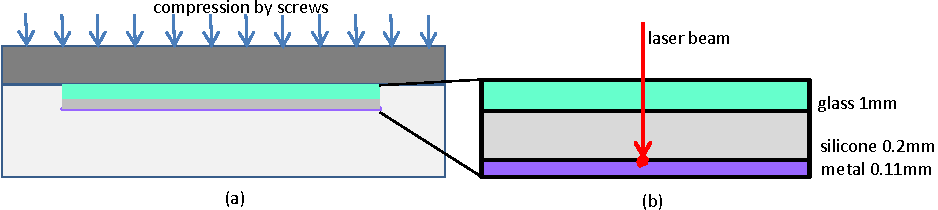
\includegraphics[width=0.8\textwidth]{figures/designandfabrication/figure3_5}%
\caption{(a) Design of the jig, (b) Thickness of each layer.}%
\label{figure3_5}%
\end{figure}

There are 5 main parameters to be set for the laser: power, frequency, speed of cutting, pulse width and number of passes. The parameter power is the power of the laser source presented with percentage to its maximum power and the speed of cutting is the moving speed of the laser beam along the processing path at the surface of the work piece as shown in \autoref{figure3_6} (a). \autoref{figure3_6} (b) illustrates the definition of frequency and pulse width. The laser pulse is a square wave and the pulse repetition rate is the parameter frequency, which is the reciprocal of the pulse period. The pulse width is the time duration in which laser beam presents. The duty ratio of the laser beam as well as the pulse period defines the average laser power with certain laser power input. In other words, longer pulse width and/or shorter pulse period (higher frequency) will result in higher average laser power.\\

\begin{figure}[b]%
\centering
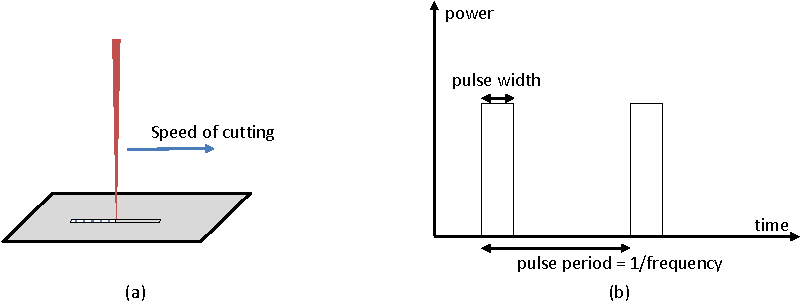
\includegraphics[width=0.9\textwidth]{figures/designandfabrication/figure3_6}%
\caption{(a) The speed of cutting is the moving speed of the laser beam along the processing path. (b) Definition of pulse width and frequency.}%
\label{figure3_6}%
\end{figure}

Each of these parameters can affect the machining quality much and these parameters interact with each other as well. To gain the optimal parameter set, the laser parameter test should be conducted at first. The laser parameter test is described as follows:\\

\begin{itemize}
	\item Two parameters are chosen as the variable for test. Here power and frequency are used as an example. Keep all the other parameters fixed.
	\item Set the range of the power and frequency.
	\item Characterize the processing quality under the microscope after machining. Choose the square with the best processing quality and record the corresponding power and frequency as shown in \autoref{figure3_7}.
	\item Switch the variable to other parameters while setting the power and frequency fixed to the former optimal value. Repeat the former steps to find all the optimal parameters which forms the optimal parameter set.
\end{itemize}

\begin{figure}[h]%
\centering
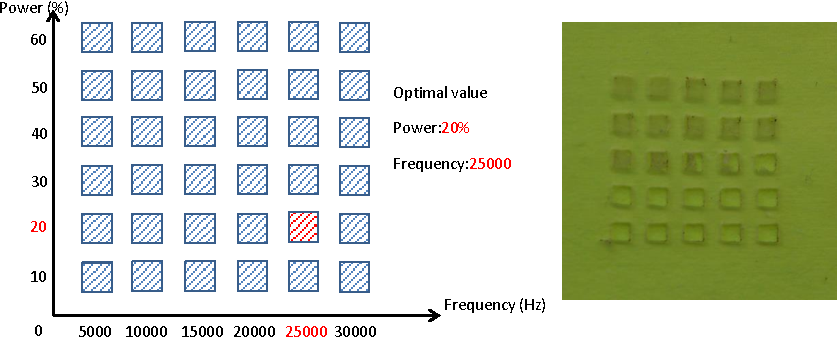
\includegraphics[width=0.9\textwidth]{figures/designandfabrication/figure3_7}%
\caption{Laser parameter test, assume the processing quality of the highlighted square is the best, the best power and frequency value is determined. Left side: schematic. Right side: test picture.}%
\label{figure3_7}%
\end{figure}

\subsection{Through-cut Microchannels}
\label{3_4_1}
The first stage of the work is to machine through-cut microchannels with surrounding additional sealing gaskets to verify the feasibility of indirect ablation and its processing quality as well. There are two possibilities to process the through-cut microchannels as shown in \autoref{figure3_8}.\\

\begin{figure}[h]%
\centering
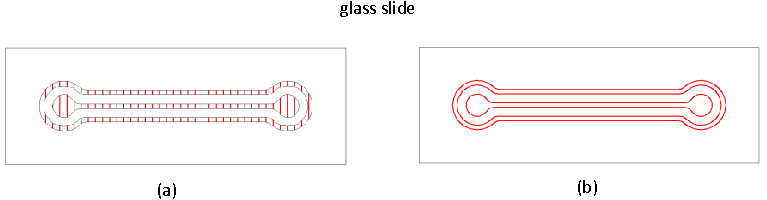
\includegraphics[width=0.9\textwidth]{figures/designandfabrication/figure3_8}%
\caption{Two methods to process through-cut microchannels. (a) Full area (red stripes represent laser cutting path) of the channel is processed. (b) Only the contour (red lines) of the channel is processed.}%
\label{figure3_8}%
\end{figure}

The first possibility is the full area scanning of the laser beam as shown in \autoref{figure3_8} (a). The filling lines represent the cutting path of the laser beam and in this way the whole area of the microchannel is ablated. However, due to the long cutting path the processing time to cut a microchannel can be more than one hour, which is of low machining efficiency. The second possibility is to only cut the contour of the microchannel as shown in \autoref{figure3_8} (b). The silicone inside the channel will still remain intact and can be peeled off after the laser processing. In this way the length of the cutting path is dramatically reduced compared to the first method and the processing time is also reduced to only around ten minutes, providing a quite efficient laser cutting. Therefore the second strategy is applied here to machine through-cut microchannels.\\

First of all, the laser parameter set is found and listed as shown in \autoref{table3_2}:

\begin{table}[!h]
    \centering
    \caption{The optimal laser parameter set for through-cut channels}
    \begin{tabular}{ll}
    \toprule
    Parameter  &   Value \\
    \midrule
    Power  &  62$\%$ \\
    Frequency  &  6900Hz \\
    Cutting speed  &  10mm/s \\
    Pulse width  &  3$\mu$s \\
    Processing passes  &  60\\
    \bottomrule
    \end{tabular}
    \label{table3_2}
\end{table}

Several different geometries of the microchannel are designed by CAD and machined by the laser. A jig is designed for the laser process. As shown in \autoref{figure3_9}, there is front window in the jig, through which the laser beam reaches the metal sheet and only this area can be processed. The four edges of the glass slide are under compression to keep the silicone membrane fixed during laser ablation. During the processing, only the outline of the microchannel is cut. \autoref{figure3_10} shows how the processing result looks like: there is a lot of black powder around the channel right after the processing and this powder is composed of both the burned metal sheet and the burned silicone membrane. After wiping these black residues away with laboratory cotton swabs the outline on the channel could be viewed clearly. The metal sheet is seriously ablated but not through-cut so that the jig is not harmed by the laser. The silicone membrane is through-cut and the channel connects the inlet and outlet reservoir. Nevertheless, the glass slide is also harmed a bit by the laser and thus it should be replaced afterwards. This transfer process will be illustrated in \autoref{3_4_3}.

\begin{figure}[ht]%
\centering
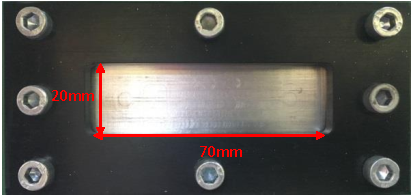
\includegraphics[width=0.5\textwidth]{figures/designandfabrication/figure3_9}%
\caption{Jig for the laser processing, the window defines the processing area.}%
\label{figure3_9}%
\end{figure}

\begin{figure}[ht]%
\centering
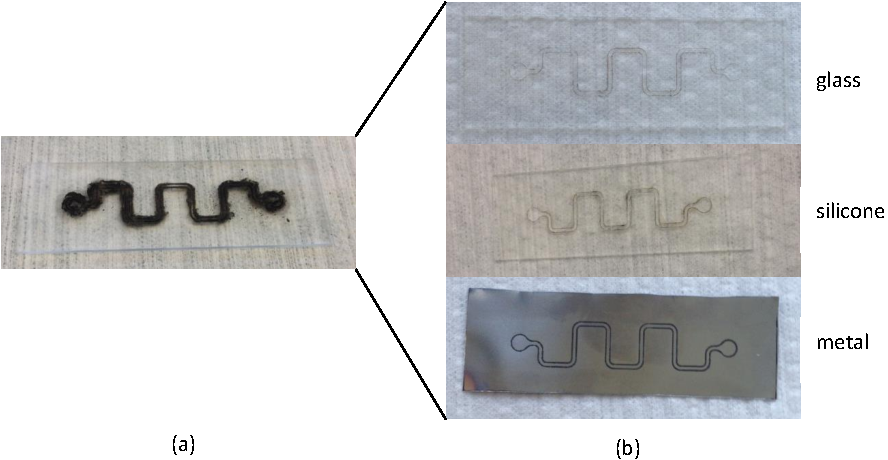
\includegraphics[width=0.95\textwidth]{figures/designandfabrication/figure3_10}%
\caption{Laser process results. (a) Before cleaning and separating the stack. (b) After cleaning and separating, silicone is through-cut, but the glass slide is also harmed by the laser.}%
\label{figure3_10}%
\end{figure}

\subsection{Flip-chip Transferring of the Silicone Microchannel}
\label{3_4_2}
For initial pressure and leakage test, through-cut microchannels with surrounding sealing gasket are needed. However, the glass slide will also get cut a bit by the laser beam as shown in \autoref{figure3_11}. As a result, this glass slide cannot be used as the mechanical carrier of the silicone membrane anymore because this cutting trace would be the weak point and even break when it is working under high pressure. Therefore the silicone membrane with microchannels built in should be transferred to a new glass slide.\\

\begin{figure}[h]%
\centering
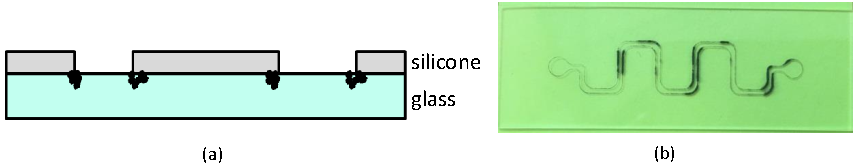
\includegraphics[width=0.9\textwidth]{figures/designandfabrication/figure3_11}%
\caption{(a) Side view of the damaged glass slide, (b) Top view of the damaged glass slide.}%
\label{figure3_11}%
\end{figure}

First of all, the front side of the silicone membrane is cleaned by ethanol. The black ablated residue should be wiped away by laboratory cotton swabs with ethanol before the transfer process. The other side of the silicone membrane which is in contact with the glass slide is also partially contaminated by the residue (black dots shown as \autoref{figure3_11} (a)) and could not be totally cleaned. It will be cleaned when the silicone is transferred to a clean slide and this surface is now exposed.\\

To glue the silicone membrane to the new glass slide the main challenge is the difficulty of obtaining a uniform thickness along the new glass slide surface, and avoiding clogging of the microfluidic channels during the curing of the adhesive. Besides, the adhesive should be optically transparent so that the view of the microchannel will not be affected by the adhesive. Since the surface energy of the silicone membrane is extremely low, only a few adhesives could thoroughly wet out the bonding interface. Besides, most adhesives such as normal adhesives (e.g. UHU Alleskleber) or epoxy based adhesives (e.g. UHU 5-Minute Epoxy) cannot glue silicone at all. Superglue (e.g. Loctite 648, Gel Sekundenkleber) is able to glue silicone, but it cures within several seconds so that there is no enough time to uniformly distribute it. And it also shrinks during curing which will cause deformation to the microchannel. At last the silicone itself is applied as the glue since it shows good compatibility to glass and to itself and will not introduce any impurities since it is the material which the silicone membrane is made from.\\

\begin{figure}[h]%
\centering
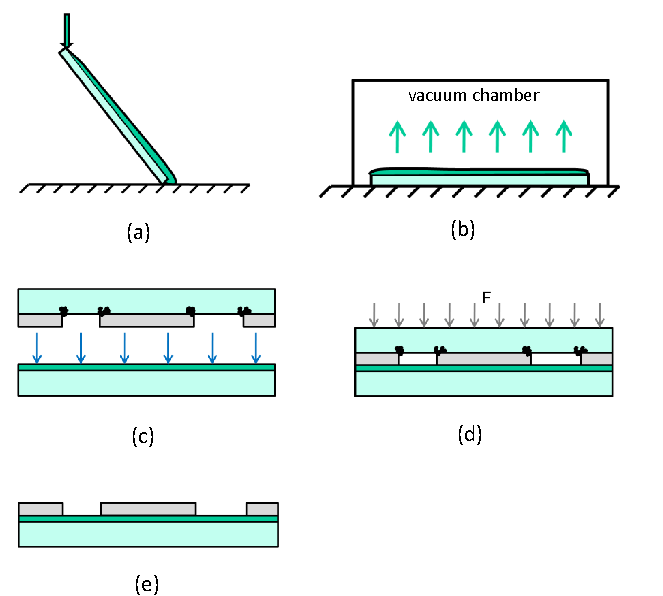
\includegraphics[width=0.8\textwidth]{figures/designandfabrication/figure3_12}%
\caption{process flow of the flip-chip transfer process of the silicone membrane.}%
\label{figure3_12}%
\end{figure}

\autoref{figure3_12} illustrates the steps transferring the silicone membrane to the new glass slide. Figure (a) shows the deposition of the glue (fluid silicone). Since the viscosity of the fluid silicone is too large for it to flow over the glass, the silicone is firstly diluted in DOW CORNING silicone solvent OS-20 \cite{os_20} to increase its fluidity. The mass mix ratio of the silicone to the solvent is 1:2. When the silicone dissolves in the solvent thoroughly by stirring, the solution is poured onto the new glass slide. To make the adhesive layer as thin as possible, which is good for a better view into the channel and does not introduce any change to the channel geometry, the glass slide is kept tilted for 1 min until most of the solution has flowed away over the glass surface and in this way a uniformly distributed thin layer of the solution is achieved. Then this glass slide is put into the vacuum chamber for degassing as shown in \autoref{figure3_12} (b). Since the OS-20 solvent is volatile, it takes only 5 min for it to evaporate. The low pressure environment in the vacuum chamber during degassing accelerates the evaporation as well. After the degassing process the patterned silicone membrane together with its original glass slide is flipped and put over the silicone covered new glass slide as shown in Figure (c). To ensure seamless contact and avoid any air bubbles, an evenly distributed compression is applied over the original glass slide by the press machine as shown in Figure (d). The pressure is kept for 2 min and then the silicone will cure within the next 12 hours. When the silicone cures, the damaged original glass slide is peeled off and the front side of the silicone membrane is cleaned. Figure (e) shows the structure of the final clean silicone membrane with intact glass slide.\\



\autoref{figure3_13} shows 4 different microchannel design sample after the flip-chip transfer process. The black residues are removed and the silicone membrane is seamlessly glued to the new glass slide without any bubbles. This process also does not change the shape of the microchannel.\\
\clearpage
\begin{figure}[h]%
\centering
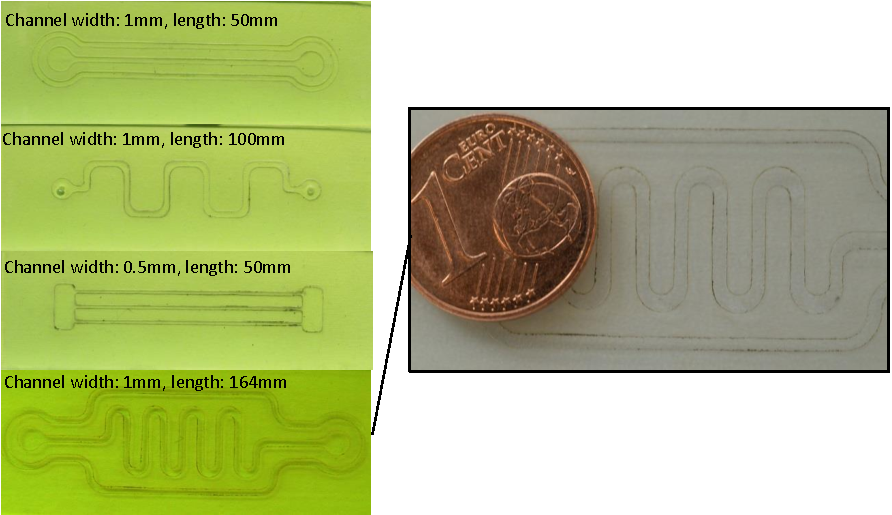
\includegraphics[width=0.9\textwidth]{figures/designandfabrication/figure3_13}%
\caption{Samples of different microchannel geometry after the flip-chip transfer process.}%
\label{figure3_13}%
\end{figure}

\subsection{Characterization of the Through-cut Microchannel}
\label{3_4_3}
After the through-cut microchannels are transferred to the clean glass slide, the processing quality is then characterized by the Laser Scanning Microscope (LSM) and the White Light Interferometer (WLI). Both results are compared for verification. Because the silicone is transparent and the reflection of the incident light from the microscope is weak, a thin layer of gold is deposited onto the silicone to enhance the reflection. \autoref{figure3_14} shows the gold coated samples.\\

\begin{figure}[h]%
\centering
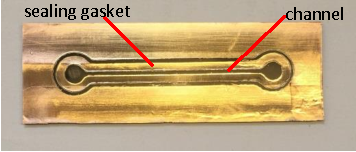
\includegraphics[width=0.5\textwidth]{figures/designandfabrication/figure3_14}%
\caption{Gold coated silicone microchannel samples, microchannel with surrounding sealing gasket.}%
\label{figure3_14}%
\end{figure}

The characterization of the microchannel is mainly the measurement of the channel depth and three-dimensional reconstruction of the microchannel. The scanning area is chosen at the channel edges, where a depth difference of 200$\mu$m should present. \autoref{figure3_15} (a) shows the channel model measured by the LSM and the depth profile across the channel. The profile gives a result of 200$\mu$m depth difference between the top surface of the silicone membrane and the channel floor, and this matches the thickness of the silicone membrane, which is 200$\mu$m. \autoref{figure3_15} (b) presents the result measured by the WLI. Likewise, the depth profile from the WLI also gives a channel depth of 200$\mu$m which matches the thickness of the silicone membrane since it is through-cut.

\begin{figure}[ht]%
\centering
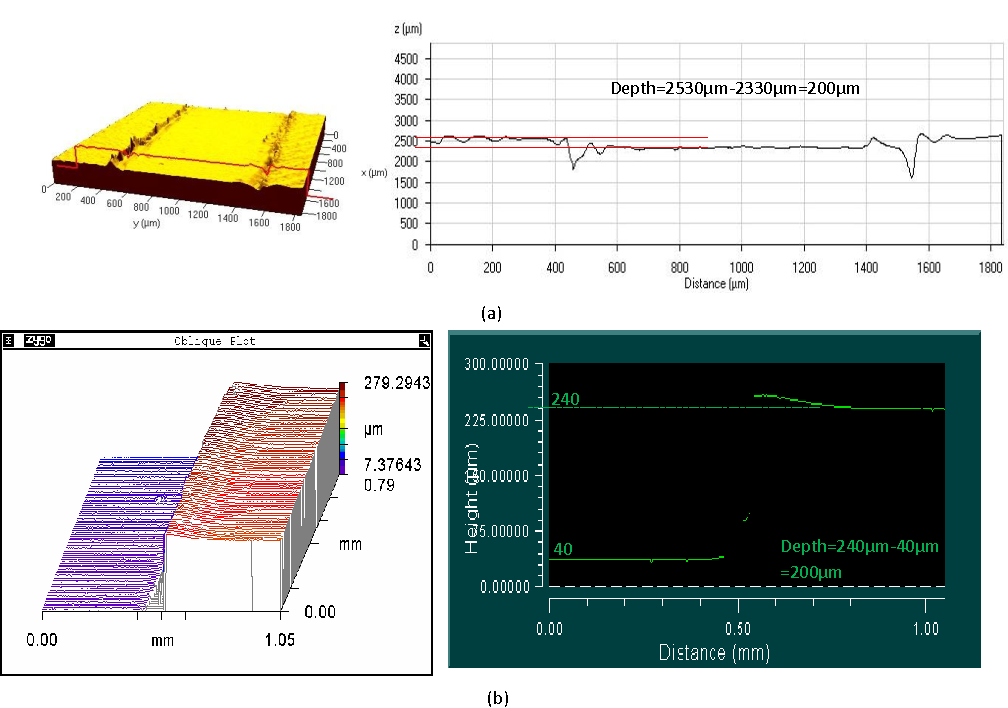
\includegraphics[width=1\textwidth]{figures/designandfabrication/figure3_15}%
\caption{(a) Result from LSM. (b) Result from WLI.}%
\label{figure3_15}%
\end{figure}

Apart from characterizing by the LSM and WLI, some directly investigated views of the channel edges are presented. \autoref{figure3_16} shows the cutting edge of straight channel. Along the edges ripples can be observed. The fluctuation of these ripples is less than 10$\mu$m, resulting in an acceptable processing accuracy.\\
\clearpage

\begin{figure}[ht]%
\centering
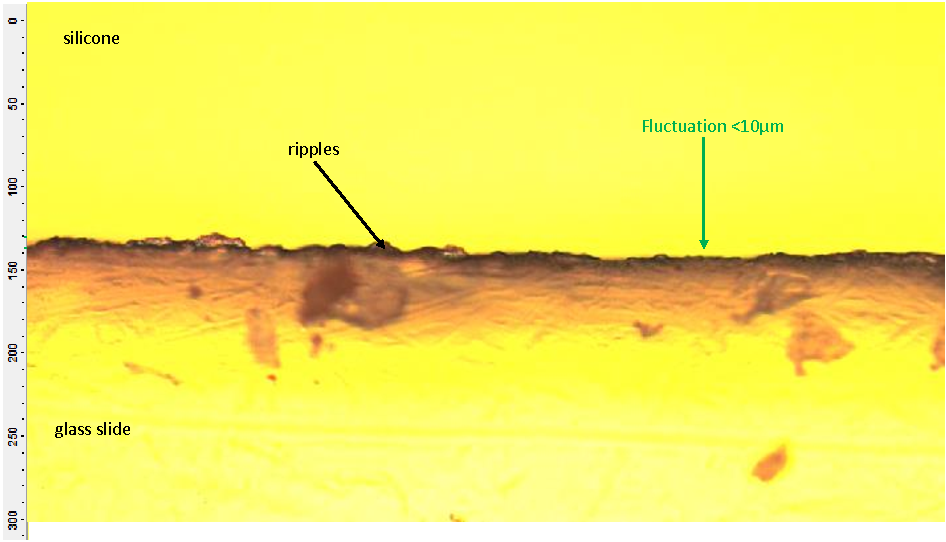
\includegraphics[width=1\textwidth]{figures/designandfabrication/figure3_16}%
\caption{Detail structure of the channel wall.}%
\label{figure3_16}%
\end{figure}

\subsection{Microchannel with Variable Depth}
\label{3_4_4}
 As illustrated in \autoref{1_2_1}, the study of bacteria adhesion features under different hydrodynamic environments are the final objective to achieve. Shear stress at the surface of the NF membrane, which may be a factor that influences bacteria adhesion, is one of these interested hydrodynamic parameters. This shear stress can be adjusted along the microchannel length by changing the depth of the microchannel. While the width of the microchannel is fixed, variation of the microchannel depth means variation of the cross-sectional area of the microchannel. Since the volumetric flow rate is fixed in a single channel test, the flow velocity will change along the length of the microchannel due to conservation of mass, leading to the variation of the shear stress on the surface of the membrane. Therefore the fabrication of microchannels with variable depth is of great interests in this master thesis work.\\

\begin{figure}[h]%
\centering
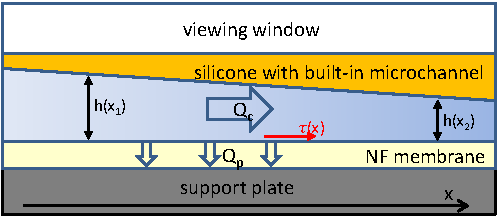
\includegraphics[width=0.6\textwidth]{figures/designandfabrication/figure3_17}%
\caption{Schematic design of integrated microchannel with variable depth.}%
\label{figure3_17}%
\end{figure}

For the through-cut channels, only the outline of the channel is cut as shown in \autoref{figure3_8}. The remaining silicone inside the channel is removed simply by the tweezers. Unlike that, all the areas in the non-through-cut channels should be processed. The channel area should be filled with stripes which are the laser cutting path rather than only processing the channel outline. \\

The laser beam is a Gaussian beam which has a waist diameter of 35$\mu$m as shown in \autoref{figure3_18} (a). This means the focused laser spot at the work piece has a diameter of 35$\mu$m. Therefore the interval of the filling lines, which are the laser scanning path, is set to 35$\mu$m as shown in \autoref{figure3_18} (b). As a result, there will not be any overlapping processing area.\\

\begin{figure}[ht]%
\centering
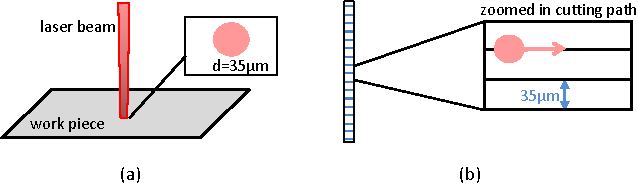
\includegraphics[width=0.8\textwidth]{figures/designandfabrication/figure3_18}%
\caption{The waist diameter of the Gaussian beam is 35$\mu$m. (b) Interval of filling lines is 35$\mu$m in order to have a smooth transition. }%
\label{figure3_18}%
\end{figure}

To find the optimal laser parameter set for a certain depth channel processing, the laser parameter tests are conducted. The test takes 6 squares as a group and only one laser parameter varies within one group. For example, when the cutting passes is under investigation, the other laser parameters are kept the same for all the 6 squares. The cutting passes increases from 20 at Square1 (S1) to 70 at Square6 (S6) as shown in \autoref{table3_3}. Therefore the cutting depth will increase from S1 to S6 and the processing quality is characterized by the microscopes.

\begin{table}[h]
    \centering
    \caption{Laser parameter set for the test}
    \begin{tabular}{ll}
    \toprule
    Other parameters & Cutting passes \\
    \midrule
    \multirow{2}{0.5\textwidth}{Speed: 10mm/s; Pulse width: 3$\mu$s; Frequency: 6900Hz; Power: 70\%} & S1: 20\ \ \ \ \ \ S2: 30\ \ \ \ \ \ S3: 40 \\
     & S4: 50\ \ \ \ \ \ S5: 60\ \ \ \ \ \ S6: 70 \\
    \bottomrule
    \end{tabular}
    \label{table3_3}
\end{table}


For the early tests, the laser power is set to a high value of 70$\%$ while the processing passes are low at 40. The other parameters are: cutting speed (10mm/s), Pulse width (3$\mu$s), Frequency (6900Hz). \autoref{figure3_19} shows the LSM picture and the WLI picture of the area which is the edge between the processed area and unprocessed area.


\begin{figure}[ht]%
\centering
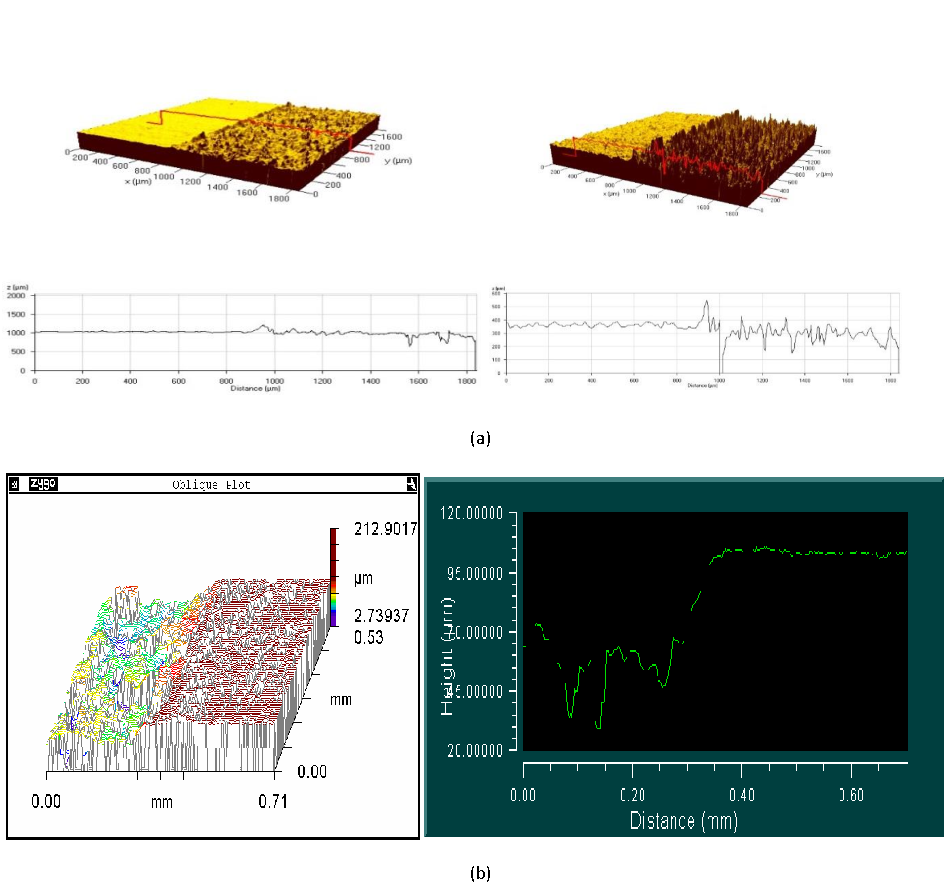
\includegraphics[width=1\textwidth]{figures/designandfabrication/figure3_19}%
\caption{(a) Processing quality picture taken by LSM. (b) Processing quality picture taken by LSM, power: 70\%, cutting speed: 10mm/s, pulse width: 3$\mu$s, frequency: 6900Hz, processing passes: 40.}%
\label{figure3_19}%
\end{figure}

From the LSM picture the cutting depth is calculated to be about 50$\mu$m, and this value matches the result measured by the WLI microscope as well. However, the surface roughness of the processed area seems to be very bad. To take a clearer view of this area and the profile in this area, this sample is also observed under the SEM as shown in \autoref{figure3_20}. The cutting depth cannot be measured by the SEM but the micro structure of the processed surface is more apparent. The silicone is ablated seriously and there are a lot of through-cut holes. Nevertheless not all the silicone is ablated which leads the processed area to be a quite porous structure. This is because the laser power is too high so that the ablated metal particles have relatively high energy which is enough to hit through the silicone membrane since the thickness of the silicone is only 200$\mu$m. Therefore the through-cut holes form. It can be predicted that if the processing passes could be increased to a proper value, all the remaining silicone will be ablated as well hence the silicone will be totally through-cut.\\

\begin{figure}[t]%
\centering
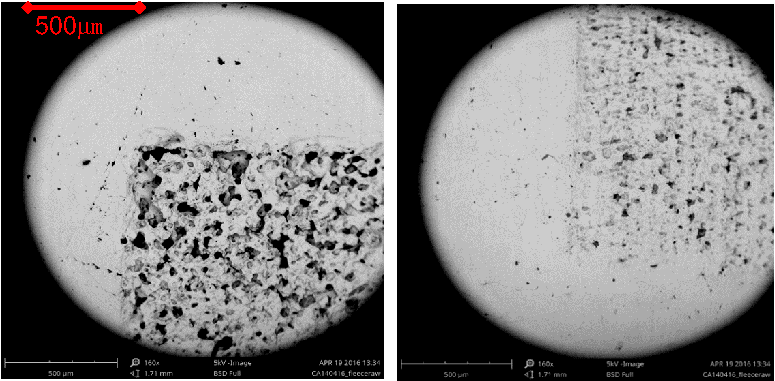
\includegraphics[width=0.9\textwidth]{figures/designandfabrication/figure3_20}%
\caption{Processing quality picture taken by SEM, power: 70, cutting speed: 10mm/s, pulse width: 3$\mu$s, frequency: 6900Hz, processing passes: 40.}%
\label{figure3_20}%
\end{figure}

\begin{figure}[!b]%
\centering
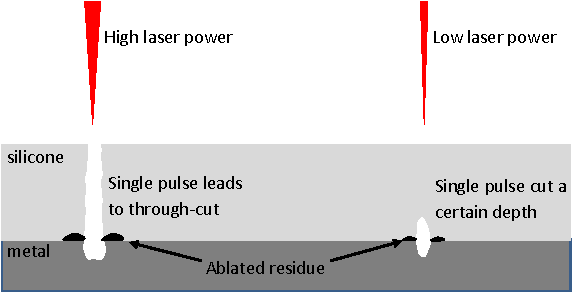
\includegraphics[width=0.6\textwidth]{figures/designandfabrication/figure3_21}%
\caption{Single laser pulse cut with high laser power and low laser power.}%
\label{figure3_21}%
\end{figure}

Since high laser power does not work for cutting silicone membrane with a certain depth, low laser power tests are conducted. As shown in \autoref{figure3_21}, with high laser power the most ablated metal particles generated by each laser pulse have the energy that is enough to penetrate the silicone membrane (these particles may have both high temperature and higher kinetic energy than that generated by low laser power). However, the energy of these metal particles will be significantly lowered down when the laser power decreases. And this energy is only enough to cut the silicone membrane a little bit each time. As a result, the cutting depth can be controlled simply by setting the processing passes. \\



Tests with low laser power are conducted with different numbers of processing passes. \autoref{figure3_22} shows the result pictures of the comparison of different processing passes taken from the LSM and SEM. From the 2 SEM pictures the cutting stripes can be observed. Picture (a) shows the result of 100 processing passes and the cutting depth is about 140$\mu$m calculated from the LSM profile. The SEM picture gives a sharply focused image of the processed area which is clean and flat and no through-cut holes present. The edge is a bit through-cut because the outline of the test square is cut for an extra time during each pass. Therefore the edge is cut for actually 200 passes and this problem is solved by excluding cutting the contour and does not present afterwards. Picture (b) shows the result of 85 processing passes and the cutting depth is about 100$\mu$m calculated from the LSM profile. Picture (c) shows the result of 70 processing passes.\\
\clearpage

\begin{figure}[!h]%
\centering
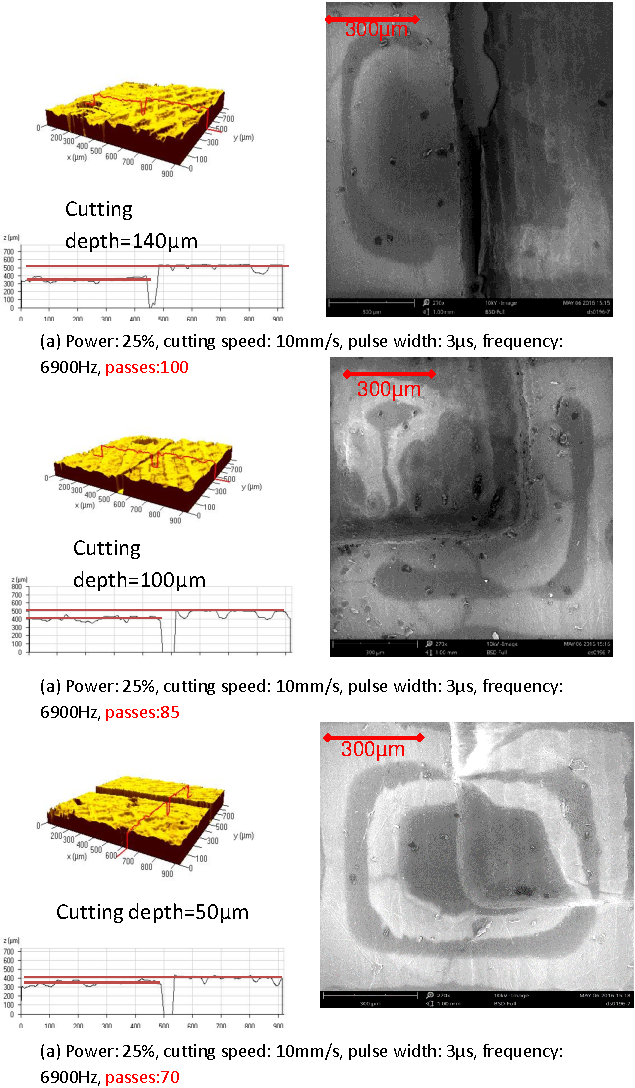
\includegraphics[width=0.82\textwidth]{figures/designandfabrication/figure3_22}%
\caption{Comparison of different processing passes with low laser power.}%
\label{figure3_22}%
\end{figure}

\clearpage

According to the data in the above Figure the cutting depth shows a linear relationship with the processing passes as shown in \autoref{figure3_22}. The linear equation is given as shown in \autoref{equation3_1}:

\begin{equation}
    d=3\times p-160
    \label{equation3_1}
\end{equation}

In this equation, d represents the cutting depth in micrometers and p represents the processing passes. However, this equation does not fit the calculation of cutting depth with low processing passes since it gives negative cutting depth with processing passes less than 50, which is impossible in reality. Therefore, the cutting depth is not correlated to the processing passes as shown in Equation 3.1 when the passes are low (at least less than 50). To characterize the relationship between the cutting depth and the processing passes with low passes, further tests need to be conducted and there might be different equations to fit to low numbers of passes, which is not done in this master thesis work.

\begin{figure}[ht]%
\centering
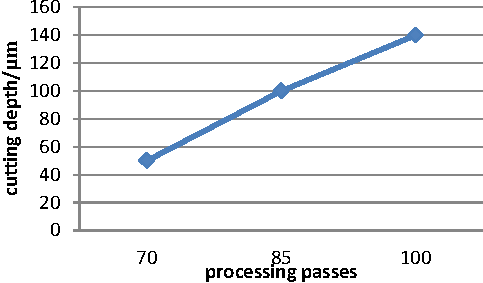
\includegraphics[width=0.55\textwidth]{figures/designandfabrication/figure3_23}%
\caption{Plot of the relationship between cutting depth and processing passes.}%
\label{figure3_23}%
\end{figure}

\begin{figure}[h]%
\centering
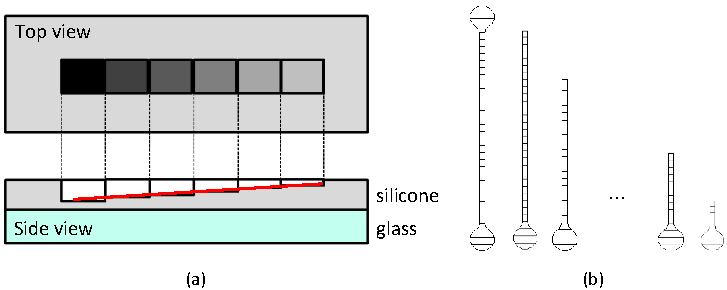
\includegraphics[width=0.8\textwidth]{figures/designandfabrication/figure3_24}%
\caption{(a) Steps with limited width can be regarded as gradual. (b) Processing mechanism of the microchannel.}%
\label{figure3_24}%
\end{figure}

\begin{figure}[!b]%
\centering
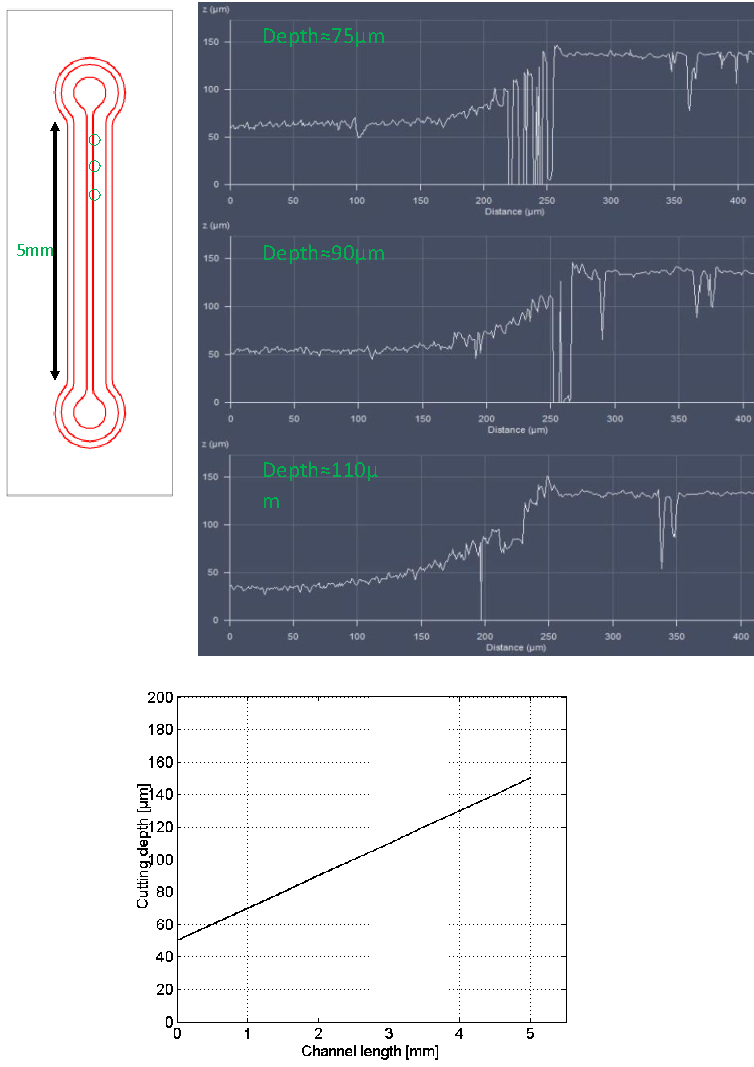
\includegraphics[width=0.9\textwidth]{figures/designandfabrication/figure3_25}%
\caption{Microchannel with variable depth.}%
\label{figure3_25}%
\end{figure}

Since it is already possible to machine microchannels with certain controllable depth in silicone membrane, a straight channel with gradual varying depth may be machined. This is done by defining steps along the length of the channel, as shown in \autoref{figure3_24} (a). In each of the step sections, the number of passes is varied, giving a varied cutting depth. If the step sections are kept relatively short, there will result a gradual continuous change in the channel height, because the laser patterning, especially by this indirect ablation method, does not yield perfect resolution.\\


\autoref{figure3_24} (b) shows the laser path to machine such channel. Firstly the total area, including the microchannel and the inlet and outlet reservoirs, is processed for 30 times as the base cycles. Then one reservoir and the microchannel are processed for 2 times as the step cycles. Afterwards the processed area is decreased gradually by decreasing 0.5mm channel length and the step cycles remain always 2. \autoref{figure3_25} shows the cutting depth measurement from the LSM.\\ 


From the figure above the change of the channel depth can be observed. The profiles are taken from different positions along the channel with the same reference plane. The channel depth varies along the channel from 75$\mu$m to 110$\mu$m. The depth of the inlet reservoir is 50$\mu$m and the depth of the outlet reservoir is 150$\mu$m. \autoref{figure3_25} shows depth profile from the start of the microchannel to the end of the microchannel and \autoref{figure3_26} shows the picture of the processed inlet reservoir and the channel.\\

\begin{figure}[ht]%
\centering
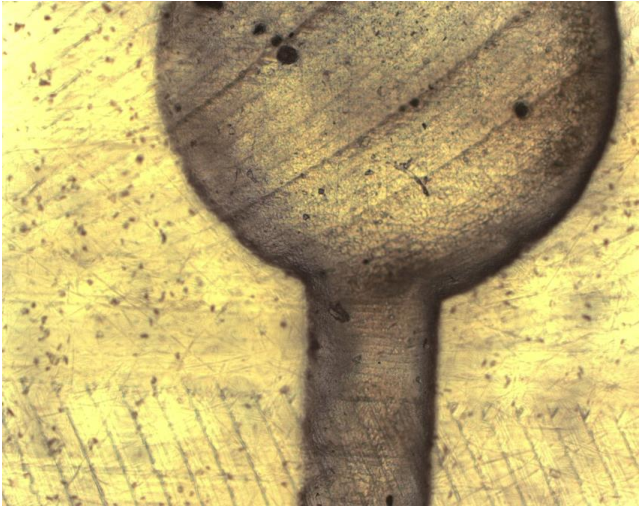
\includegraphics[width=0.6\textwidth]{figures/designandfabrication/figure3_26}%
\caption{Part of the microchannel with variable depth.}%
\label{figure3_26}%
\end{figure}

\clearpage

\section{Design and Fabrication of the Chip Housing}
\label{3_5}
The microfluidic platform in this thesis work is designed for testing the performance of the nanofiltration membrane and the adhesion and deposition features of bacteria on it. As shown in \autoref{figure3_27}, the silicone microchannel is designed for the suspension to flow through under high pressure. When the suspension flows over the nanofiltration membrane, it also permeates through the nanofiltration membrane which forms the permeate flow $Q_p$. The bacteria adhesion to the NF membrane should then be studied under the effect of this permeate flow. Furthermore, the shear stress along the channel length will change due to the change of channel depth and it is also of interest to study the contribution to the bacteria adhesion made by the shear stress. The initial housing design is to mount the silicone microchannel and keep it well sealed for the pressure and leakage test. Then the nanofiltration membrane need also be assembled into the housing. In this section, three designs are shown. The first design is simply to test the pressure bearing capacity of the silicone microchannel. The second design is improved based on the first design. The third design is the final housing design containing the nanofiltration membrane, which required a modification of the inlet and outlet configuration.\\

\begin{figure}[ht]%
\centering
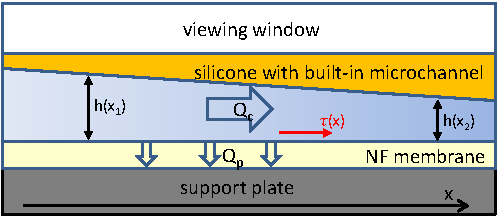
\includegraphics[width=0.6\textwidth]{figures/designandfabrication/figure3_27}%
\caption{Design concept of the microfluidic platform}%
\label{figure3_27}%
\end{figure}

\subsection{Housing Design 1}
\label{3_5_1}
In this design the fluid flows simply through the microchannel under high pressure. The fluid is pressurized by a pressure accumulator which is illustrated in \autoref{3_6}. The housing must be able to withstand high pressure at least up to 10bar. The glass slide, as the mechanical carrier of the silicone membrane, must also remain intact under such pressure and the fluid should not leak to anywhere other than the microchannel.

\begin{figure}[!h]%
\centering
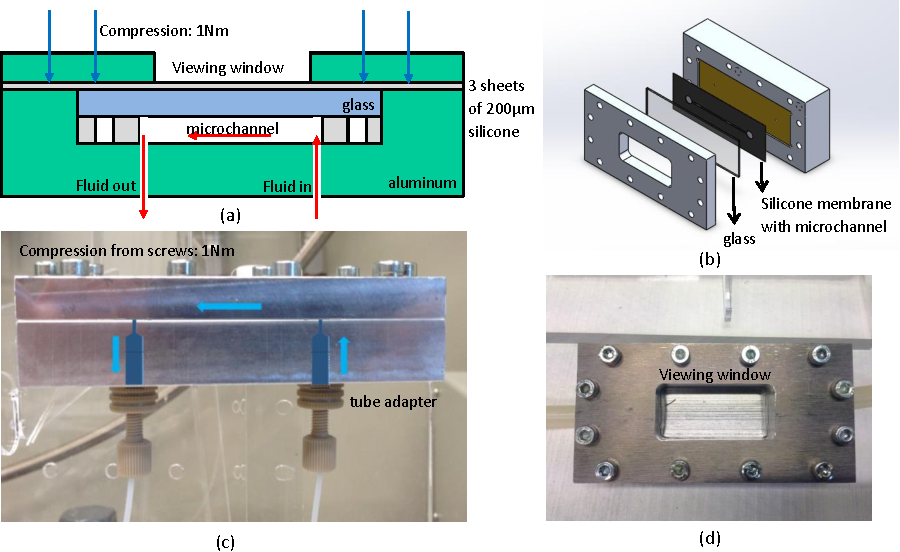
\includegraphics[width=1\textwidth]{figures/designandfabrication/figure3_28}%
\caption{Schematic of the housing design 1 and the finished product. (a) Side view of the schematic of the housing design. (b) Isometric view of the assembly of the housing design. (c) Side view of the finished product. (d) Top view of the finished product.}%
\label{figure3_28}%
\end{figure}

As we can see in \autoref{figure3_28} the silicone membrane together with the glass slide is pressed against the base plate of the housing. In this way the microchannel is sealed by the seamless contact between the silicone membrane and the base plate. The inlet and the outlet are placed at the bottom side so that fluid can directly enter the microchannel. A metal lid is connected to the base plate by 12 screws to provide compression to the glass slide for sealing. However, in this case the compression lies on the four edges of the glass slide and the center of the glass slide is not compressed, resulting in a non-uniform distributed compression force. To avoid direct contact of the metal lid and the glass slide and also to achieve a more evenly compression distribution, 3 layers of silicone membranes are placed in between to provide a cushion room since metal and glass are both rigid materials. There is a window in the middle of the metal lid in order to observe the microchannel from the top side. The screws are tightened by the torque wrench and the torque is set to 1N$\cdot$m.

\subsection{Housing Design 2}
\label{3_5_2}
\begin{figure}[t]%
\centering
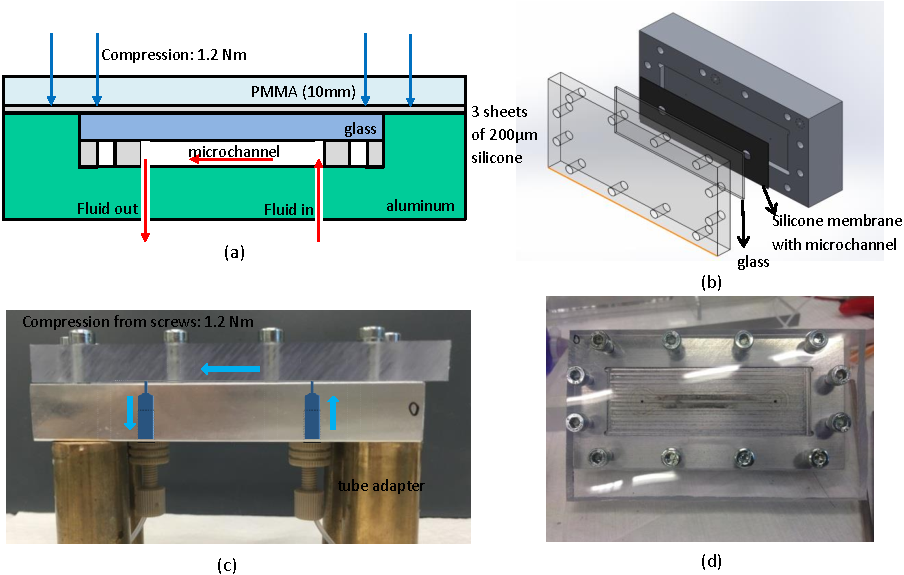
\includegraphics[width=1\textwidth]{figures/designandfabrication/figure3_29}%
\caption{Schematic of the housing design 2 and the finished product. (a) Side view of the schematic of the housing design. (b) Isometric view of the assembly of the housing design. (c) Side view of the finished product. (d) Top view of the finished product.}%
\label{figure3_29}%
\end{figure}

In the former housing design the lid is made from aluminum and the viewing window is in the middle of this lid. The glass slide is pushed against the base plate by the metal lid. However, the force bearing area on the glass slide is at the four edges, and that leads to a non-uniform force distribution. Therefore the glass slide broke easily when the screws were tightened and even though it was successfully assembled, cracks appeared at the inlet and outlet at the pressure of only 1 bar. Moreover, the viewing window is also not large enough to show the whole channel and the inlet and outlet reservoirs.\\

To solve these problems, the aluminum lid is replaced by a PMMA lid. Since PMMA is totally transparent, it needs not to be cut in the middle for the viewing window and this time a full view of the microchannel can be achieved. Another advantage of using PMMA lid is that the glass slide is in full contact with the lid so that the compression force distribution is quite uniform over the full slide surface. Hence the glass slide will not break easily. \autoref{figure3_29} shows the schematic design and the finished product of housing design 2.

\subsection{Housing Design 3}
\label{3_5_3}
\begin{figure}[t]%
\centering
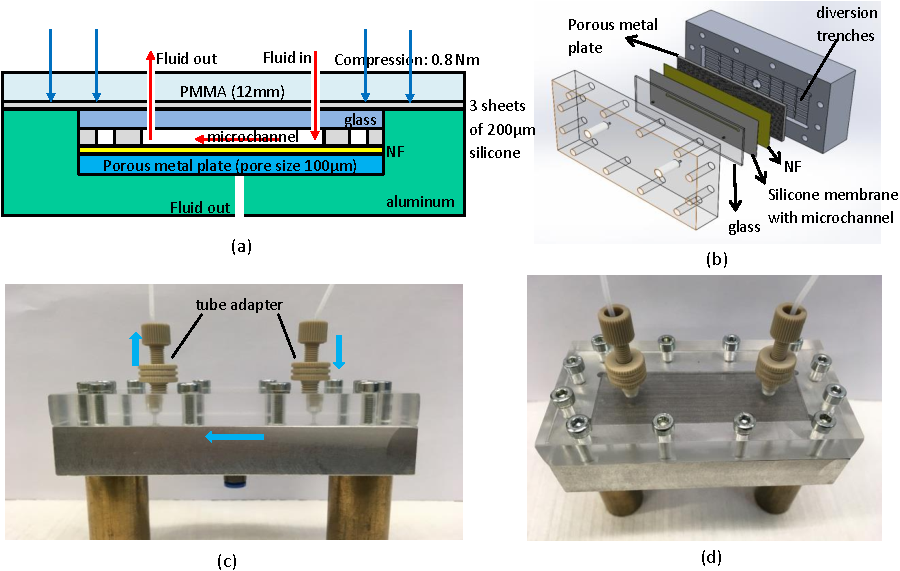
\includegraphics[width=1\textwidth]{figures/designandfabrication/figure3_30}%
\caption{Schematic of the housing design 3 and the finished product. (a) Side view of the schematic of the housing design. (b) Isometric view of the assembly of the housing design. (c) Side view of the finished product. (d) Top view of the finished product.}%
\label{figure3_30}%
\end{figure}

The former designs are targeted at testing the highest pressure that the microchannel can withstand so that the NF membrane is not taken into account. In this design, the aim is to assemble all the parts including the microchannel and the NF membrane inside. \\

\autoref{figure3_30} (a) shows the schematic design. The silicone membrane with built in microchannel sits on top of the NF membrane so that the fluid can flow over the NF membrane. Since the thickness of the NF membrane is only 160$\mu$m and it can deform easily, a support plate need to be placed underneath. This support metal plate is made of stainless steel and is porous so that the fluid which permeates the NF membrane could flow out through the outlet hole at the bottom of the housing. The pore size of the porous metal plate is 100$\mu$m and water can permeate this plate with minimal resistance.\\

In this housing design the fluid should not be loaded in to the channel from the bottom side since the NF membrane needs to be intact and sealed against the silicone gasket. As a result, the inlet and outlet interfaces are placed at the top side. The PMMA lid is drilled with threaded holes to assemble the tube adapters as shown in \autoref{figure3_30} (c). Two holes for the inlet and outlet are also drilled in the glass slide to let the fluid flow through. The diameter of these two holes is 1.1mm. There are also interlaced diversion trenches designed beneath the porous metal plate in the aluminum housing to let the permeated fluid to flow out as shown in \autoref{figure3_30} (b). \autoref{figure3_30} (c) and (d) show the finished product of the design.\\ 

For drilling the inlet and outlet holes in the glass slide was to build a stack of glass slides. The chip (glass slide with the patterned silicone membrane) is covered by two layers of sacrificial glass slides of the same size as shown in \autoref{figure3_31} (a). This stack is fixed by colophony, which melts at 120$^\circ$C and solidifies at room temperature, so that the glass slides will not move during drilling. Then the colophony is removed from the stack and the chip is taken out and cleaned by ethanol (colophony dissolves in ethanol).

\begin{figure}[!t]%
\centering
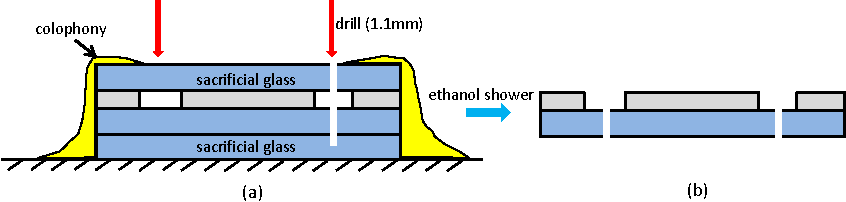
\includegraphics[width=1\textwidth]{figures/designandfabrication/figure3_31}%
\caption{Glass drilling process. (a) The chip is covered by two sacrificial glass slides and fixed by colophony. (b) Colophony is cleaned by ethanol.}%
\label{figure3_31}%
\end{figure}

\begin{figure}[!t]%
\centering
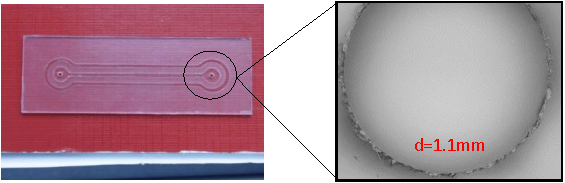
\includegraphics[width=0.7\textwidth]{figures/designandfabrication/figure3_32}%
\caption{Microscopic view of the drilled holes in glass slide.}%
\label{figure3_32}%
\end{figure}
\autoref{figure3_32} shows the microscopic view of the holes in the glass slide. The glass slide does not break during the drilling process and no cracks present as well.

\clearpage

\section{Design of the Test Setup}
\label{3_6}
As discussed in previous sections, the main goal is to test the working performance of the microchannel and the NF membrane under high pressure. In this section, the test setup is designed to pressurize the fluid and load it into the microchannel.\\

A pressure accumulator is designed to pump fluid into the microfluidic platform as shown in \autoref{figure3_33}. The pressure accumulator is made of aluminum and it has a wall thickness of 18.82mm. It is sealed by 6 O-rings, 2 O-rings used for the movable piston to separate the nitrogen and loaded water and 4 O-ring used to seal the both lids. In this way the high pressure nitrogen gas can be used to pressurize the housing. 

\begin{figure}[ht]%
\centering
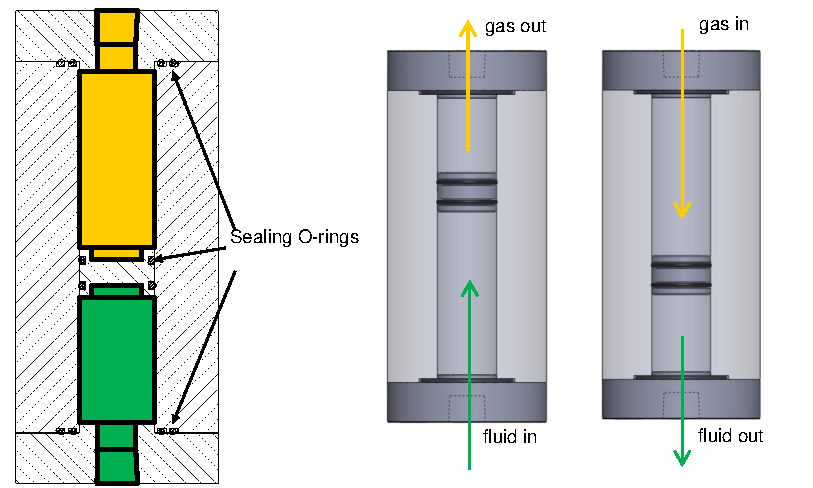
\includegraphics[width=0.8\textwidth]{figures/designandfabrication/figure3_33}%
\caption{Schematic and working principle of the pressure accumulator.}%
\label{figure3_33}%
\end{figure}

\autoref{figure3_34} shows the schematic design of the test setup with housing design 2. A pressure regulator with a relief valve set at 50bar is used to apply pressure to a piston in the pressure accumulator, which drives the flow into the microchannel. A syringe is connected to the canister and the piston will be pushed upwards to load fluid into the canister. Two pressure sensors (PS) with accuracy of 0.6bar are installed to measure both, the fluid pressure before it enters the microchannel and the fluid pressure it flows out of the microchannel. The measurements are made every 1ms and the data acquisition device (NI-USB 6008 from National Instruments) transfers the pressure measurements to a PC, where the data is analyzed and stored. A back pressure regulator (BPR) is also installed to keep the pressure inside the microchannel to a set value.\\
\clearpage
\begin{figure}[ht]%
\centering
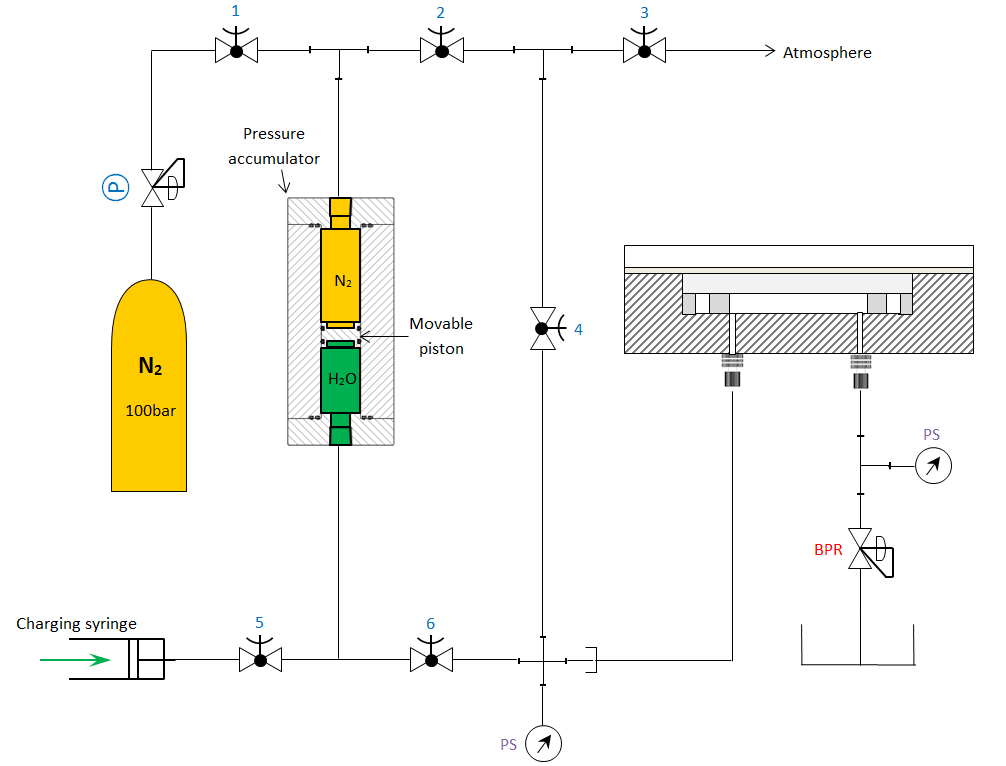
\includegraphics[width=1\textwidth]{figures/designandfabrication/figure3_34}%
\caption{Schematic of the test setup design.}%
\label{figure3_34}%
\end{figure}



\noindent \textit{Loading fluid to the pressure accumulator}\\

Consider that all the valves are closed. By opening the valves 2, 3 and 5 the fluid can be pre-loaded into the pressure accumulator. This is done by using a syringe coupled to valve 5 and by pushing the syringe the movable piston will be pushed upwards, repelling the gas out of the canister and thus fluid is loaded as shown in \autoref{figure3_35}. Once the fluid is loaded to the pressure accumulator, the valve 2, 3 and 5 must be closed in order to keep the fluid inside the system.\\
\clearpage

\begin{figure}[ht]%
\centering
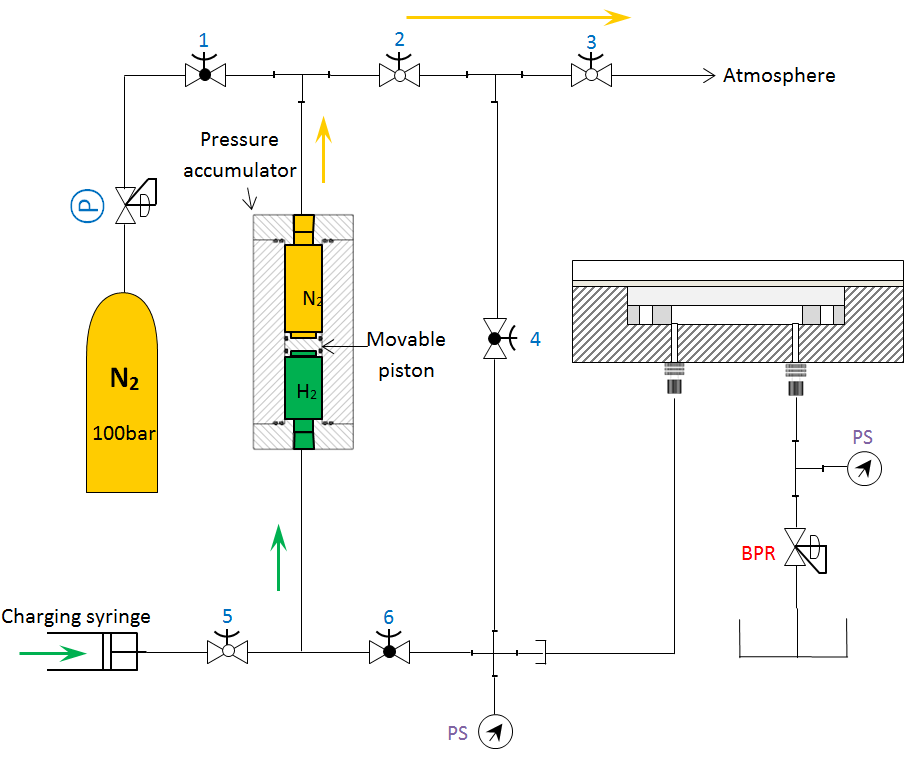
\includegraphics[width=0.8\textwidth]{figures/designandfabrication/figure3_35}%
\caption{Loading fluid into the pressure accumulator.}%
\label{figure3_35}%
\end{figure}

\noindent \textit{Pumping the fluid into the microfluidic platform}\\

Consider that all the valves are closed. By opening the valves 1 and 6 the nitrogen will flow from the high pressure nitrogen tank to the pressure accumulator and cause downward displacement of the piston, which pumps the fluid into the microfluidic platform. Since the BPR only releases pressure when the pressure is higher than its set value, the pressure regulator at the high pressure nitrogen tank should be set at a pressure higher than the BPR can withstand.\\
\clearpage

\begin{figure}[ht]%
\centering
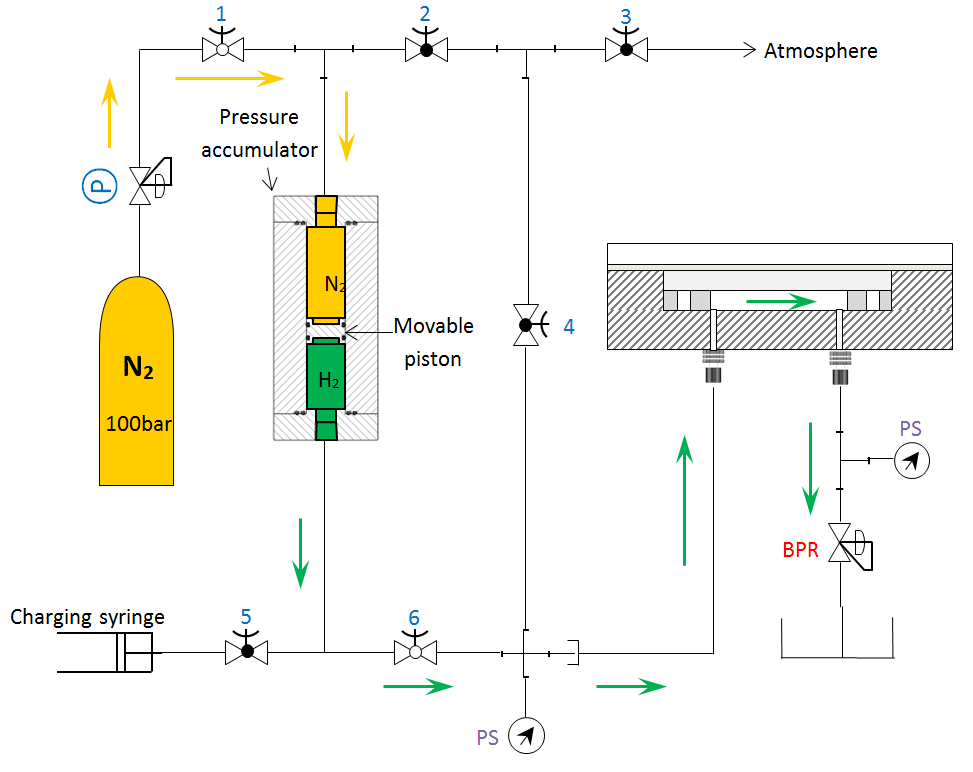
\includegraphics[width=0.8\textwidth]{figures/designandfabrication/figure3_36}%
\caption{Pumping the fluid into the microfluidic platform.}%
\label{figure3_36}%
\end{figure}

\noindent \textit{Purging the microchannel}\\

Consider that all the valves are closed. By opening the valves 1, 2 and 4 the nitrogen will flush into the microchannel and thus the flow loop is purged.\\
\clearpage

\begin{figure}[!h]%
\centering
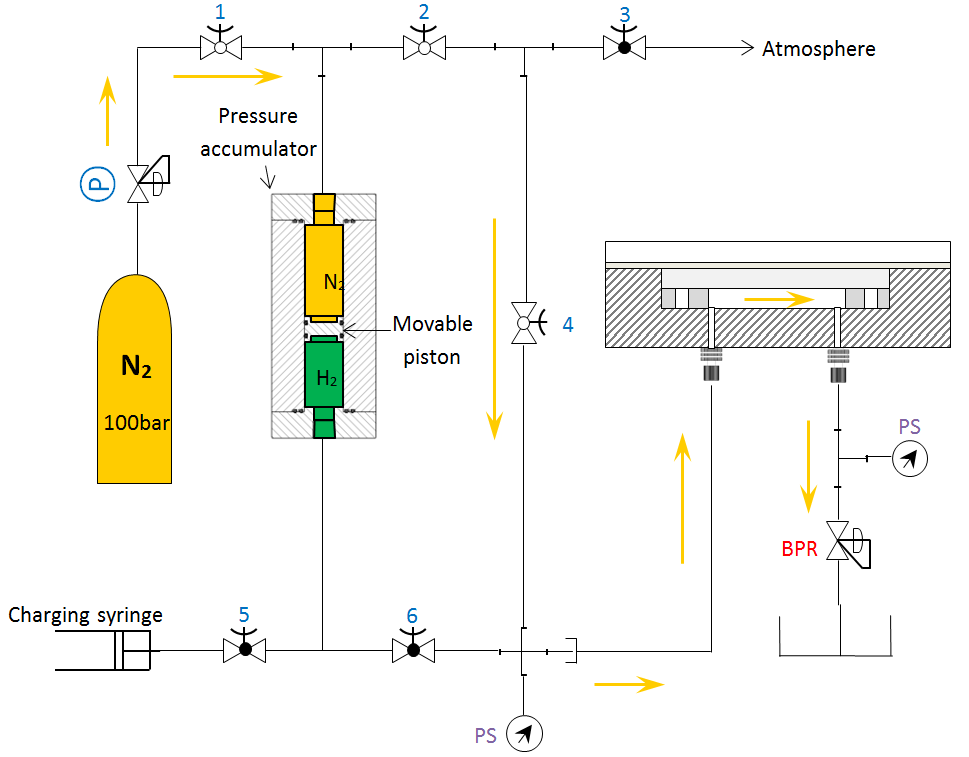
\includegraphics[width=0.8\textwidth]{figures/designandfabrication/figure3_37}%
\caption{Purging the microchannel.}%
\label{figure3_37}%
\end{figure}




